\documentclass[a4paper,12pt]{article}

\usepackage{fancyhdr}
\usepackage{lastpage}
\usepackage{amsmath}
\usepackage{tikz}
\usepackage{amsfonts}
\usepackage{csvsimple}
\usepackage{graphicx}
\pagestyle{fancy}

\lhead{Samuel Loomis}
\setlength{\headheight}{15pt}
\chead{PH 411 Lab1}
\rhead{\thepage\ of \pageref{LastPage}}
\lfoot{}
\cfoot{}
\rfoot{}

\begin{document}
\section*{Experiment 1}
Measuring the resistance of a single resister at a single voltage setting will not allow us to tell if the resisor is ohmic or not.  More data is required.

The voltage must be varried and data for the current and voltage across the resistor collected to find out if it is an ohmic resistor.

A standard circuit (see circuit: Resistor) was set up.  The voltage was varried and data collected (see table: 1c).\\
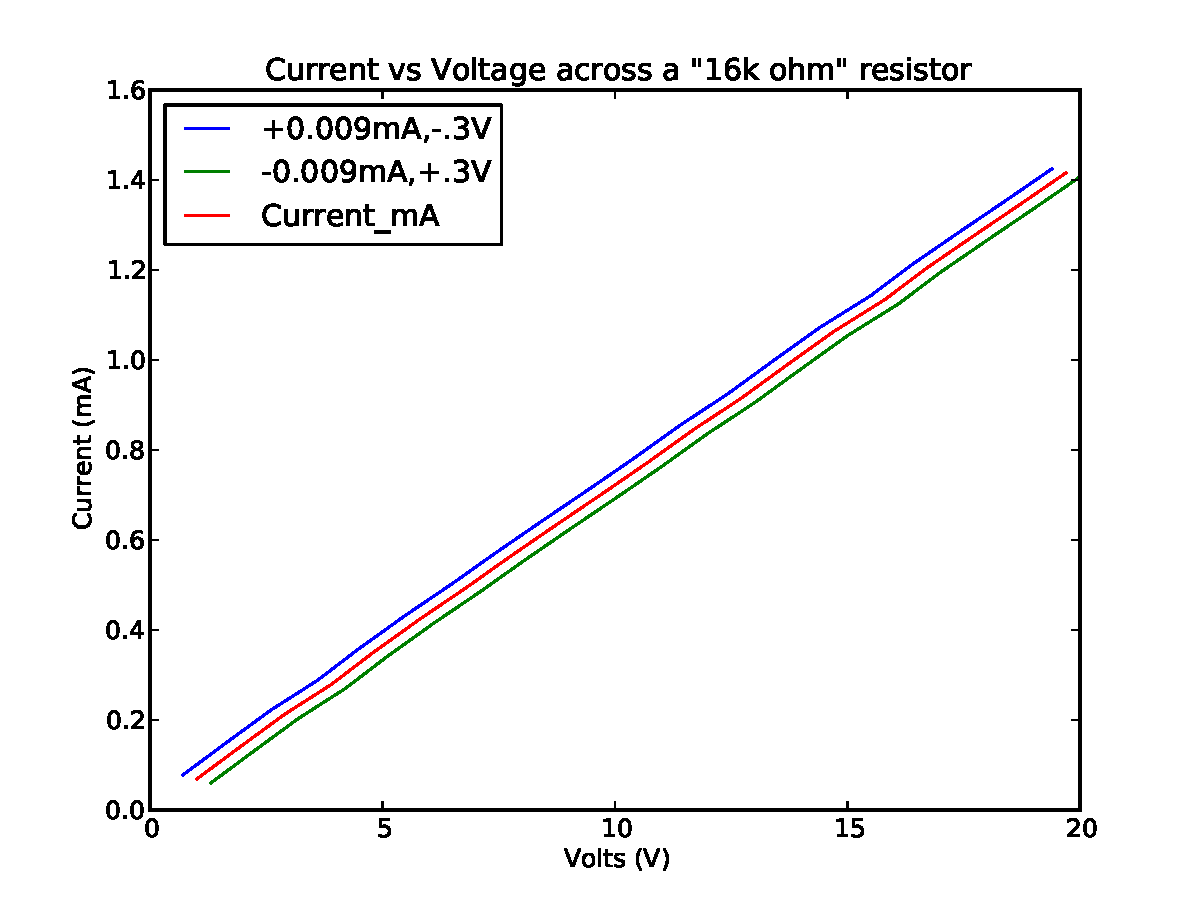
\includegraphics[width=6in]{411labp1.pdf}\\
As one can see, the graph is quite linear.  The blue line is maximizing the error above the data collected and the green line maximizes the error below.  According to this data, the resistor is between 13.6 and 14.2 k$\Omega$.  The resistor color code was Red Blue Orange Gold, which equates a $16\pm5\%k\Omega$ resistor.  This equates to a resistor range of 15.2-16.8k$\Omega$.  There is some sort of error missing, possibly internal resistances in our measurement devices?

Data was also collected for the resistor at varying temperatures. (see table: 1d)  According to this data, the resistance didn't vary much with temperature at all.  The resistance read at 115 to 116$\Omega$ between the entire range of temperatures from -7$^\circ$C to 50$^\circ$C.  The error in the measurement was $\pm$3$\Omega$.  Thus the measurement varying was within the error values the entire time, and the resistor can be considered constant.

A thermister was checked to compare to a regular resistor.  (see table: 1e)\\
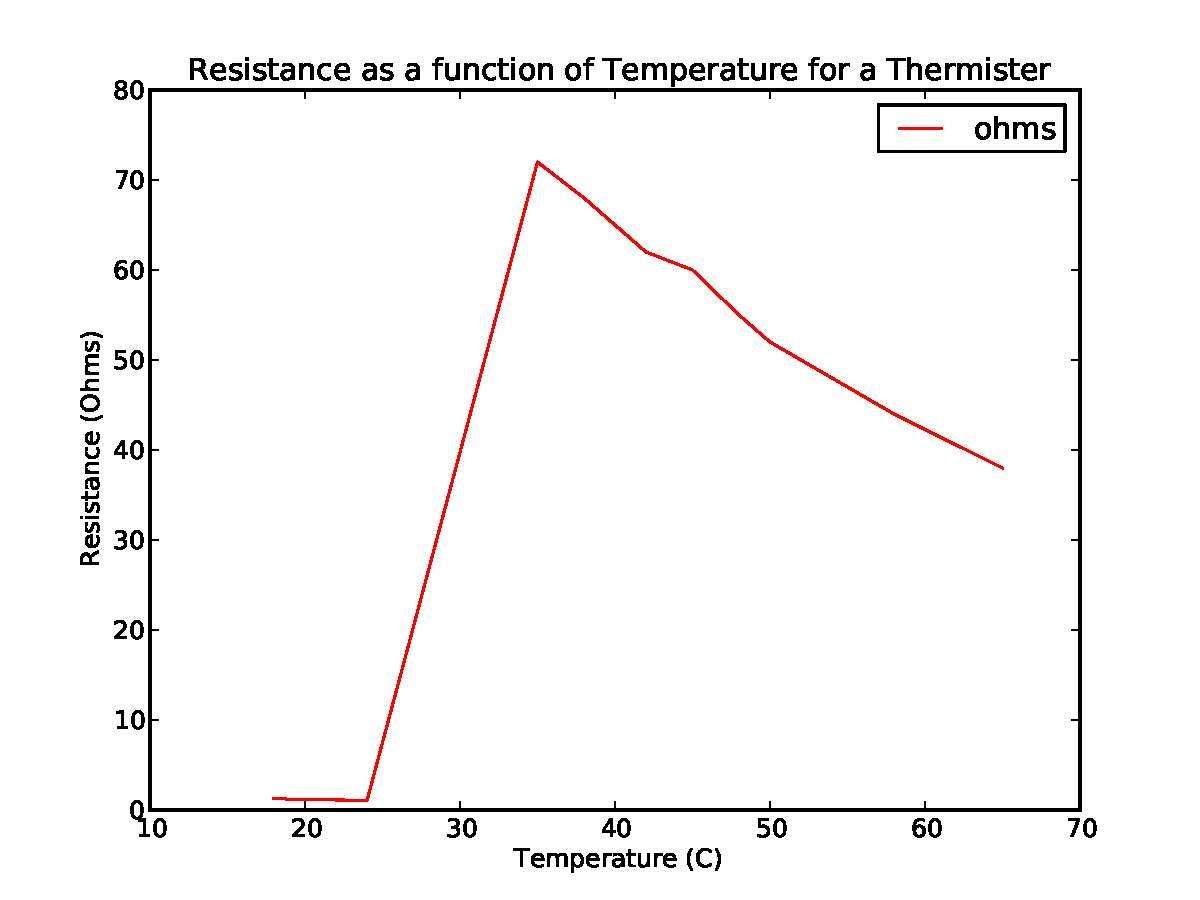
\includegraphics[width=6in]{411labp1e.pdf}\\
Currently, I think the data is corrupted, I need to verify with my lab partner.  I expected to see a decreasing resistance as temperature increased.  The graph tends to follow that trend, but possibly human error in documenting the resistance values occured.

\section*{Experiment 2}
This experiment tests the resistivity of objects other than resistors. (see circuits: Graphite, Diode and LED)\\*
First a small diameter graphite rod was tested. (see table: 2a Small Rod)\\*
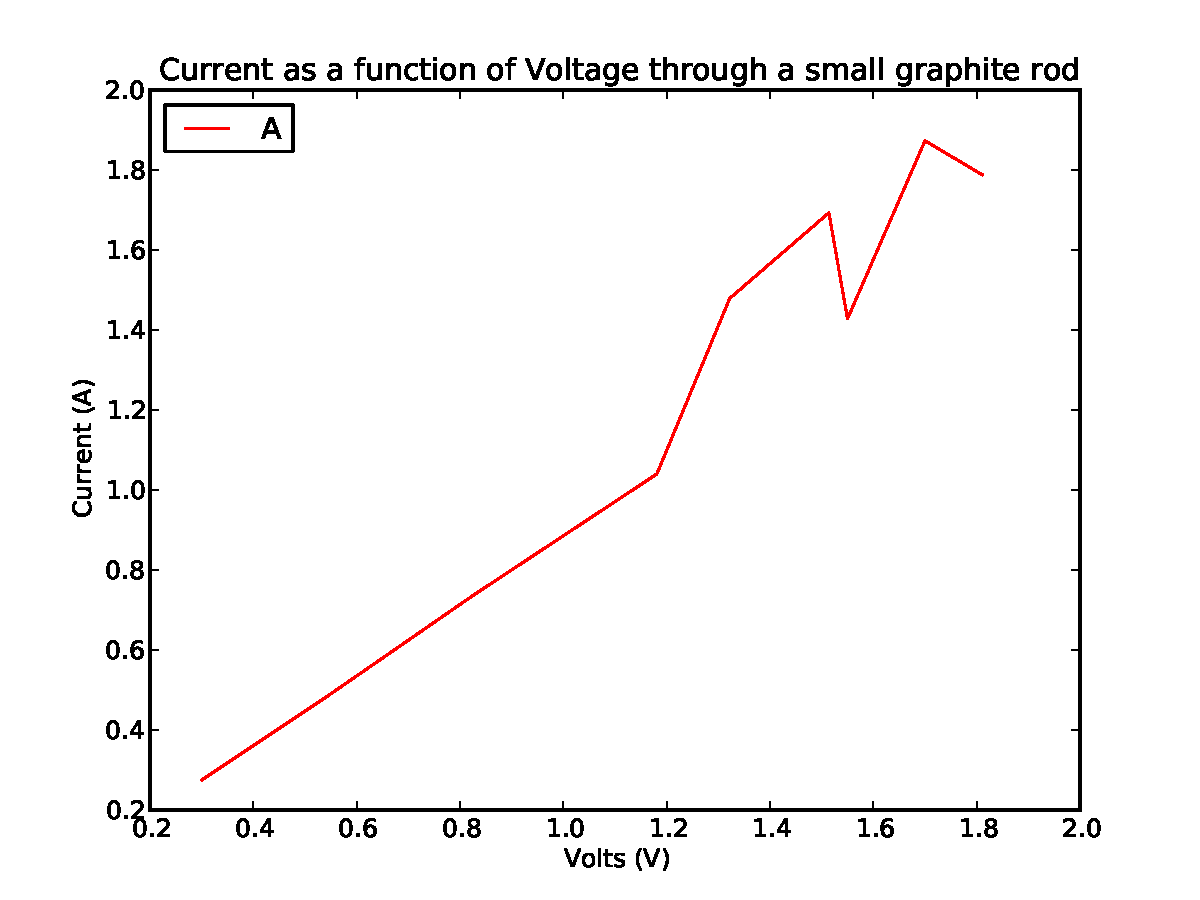
\includegraphics[width=6in]{411labp2asmall.pdf}
Then a larger diameter graphite rod was tested. (see table: 2a Big Rod)
Data was then collected for two types of diodes. (see tables: 2b and 2c)
(Data still needs to be collected for burning out the LED. Likely collect it on monday around noon, after capstones.)

\section*{Experiment 3}
A circuit to test potential dividers was set up. (see circuit <name>)

Resistor 2, the one the potential was checked across was varried from 200$\Omega$ to 1M$\Omega$.  (see table <name>)

The same types of measurements were done starting with 16k$\Omega$ of each resistor, then varying resistor 2 again. (see table <name>)

\section*{Experiment 4}

To gain the knowledge needed to find internal resistances ($R_{int}$)\ and internal voltage ($V_{int}$) ($V_{th}$) or Thevenin voltage) a complex circuit was created. (see circuit <name>)  Using this circuit, the voltage across the far terminal ($V_{th}$) simulates the voltage we see from a powersupply.  The power supply has an internal resistance, and using the methods learned in this experiment, they can be analyzed and found.

(Calculated values to be inserted here)

\section*{Experiment 5}

Using the Tevenin analysis from Experiment 4, the internal resistances of the DC power supply and the DMM measurement devices can be obtained.  (see table <name>)
(the internal resistance of the dmm still needs to be found, will take that data when the data is collected for the diode.)

\section*{Assigned Problems}
\subsection*{1.15}
A gas discharge tube draws a current of 20mA while maintained in a 800V potential drop.  What is the effective DC resistance in ohms?\\
\begin{align*}
R=?\ \ &V=800 V\ \ I=0.02 A\\
V&=IR\ \ \ R=\frac{V}{I}\\
R&= \frac{800 V}{0.02 A}\\
R&= 40.k\Omega
\end{align*}
\subsection*{1.18}
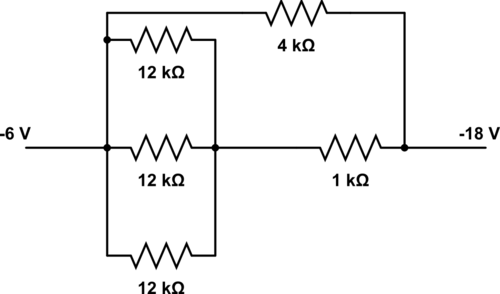
\includegraphics{1_18-circuit.png}\\
Find the current flowing through the ends,(marked I in the book pg 49, left out on this diagram).\\*
\\*
The circuit shown can be simplified to 1 resistor with a voltage drop across it.  The current through the entire circuit will be equal to $I=\frac{V}{R}$, where $V=-18V-(-6V)=-12V$ and $R=R_{eq}$.
Finding $R_{eq}$:
\begin{align*}
R_{eq} &= \frac{1}{\frac{1}{4k\Omega}+\frac{1}{1k\Omega+\frac{1}{\frac{1}{12k\Omega}+\frac{1}{12k\Omega}+\frac{1}{12k\Omega}}}}\\
R_{eq} &= \frac{1}{\frac{1}{4k\Omega}+\frac{1}{1k\Omega+4k\Omega}}\\
R_{eq} &= \frac{1}{\frac{1}{4k\Omega}+\frac{1}{5k\Omega}}\\
R_{eq} &= \frac{1}{\frac{5}{20k\Omega}+\frac{4}{20k\Omega}}\\
R_{eq} &= \frac{20k\Omega}{9}\\
R_{eq} &= 2.\overset{\_}{2}k\Omega\\
R_{eq} &\approx 2k\Omega
\end{align*}
Finding Current:
\begin{align*}
I &= \frac{V}{R_{eq}}\\
I &= \frac{-12V}{2.\overset{\_}{2}k\Omega}\\
I &= -5.4A
\end{align*}
\subsection*{1.27}
On a microscopic basis, when electical energy flows through a resistor, the molecules of the resistor get excited and convert energy into random thermal energy.  If current is flowing through a resistor, it is generating heat.  The amount is based on how much power it is actually disipating.
\subsection*{1.30}
From inside section 1.6 in the simpson book...  The maximum power disipated is achieved when $R_h=R_{int}=3\Omega$.  Finding it is as follows:
\begin{align*}
P_h &= IV_h\\
I = \frac{V_{bat}}{r+R_h}\ &\ V_h=IR_h=\left(\frac{V_{bat}}{r+R_h}\right)R_h\\
P_h &= \left(\frac{V_{bat}}{r+R_h}\right)^2R_h\\
\text{Taking the derivative:}&\\
\frac{\partial P_h}{\partial R_h} &= V_{bat}^2\frac{(r+R_h)^2-2R_h(r+R_h)}{(r+R_h)^4}\\
\text{Setting the derivative to}\ &\text{0 and solving for} R_h:\\
0 &= \frac{V_{bat}^2}{(r+R_h)^4}[(r+R_h)^2-2R_h(r+R_h)]\\
(r+R_h)^2 &= 2R_h(r+R_h)\\
R_h^2+2rR_h+r^2 &= 2rR_h+2R_h^2\\
r &= R_h
\end{align*}
The power dissipated across the heater and in the battery are both equal:
\begin{align*}
P_{bat} = P_h &= \frac{V_h^2}{R_h}\\
P_h &= \frac{(6V)^2}{3\Omega}\\
P_h &= 12 W
\end{align*}
\subsection*{1.32}
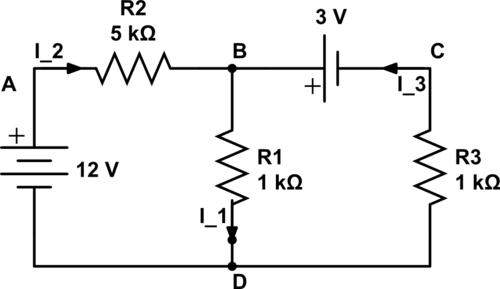
\includegraphics{1_32.png}\\
Analyzing the circuit, considering point D is ground. Values for I are in mA and values for R are in k$\Omega$:
\begin{align*}
I_1 - I_2 = I_3&\\
12V-I_2R_2-3V+I_3R_3 &= 0V\\
12V-I_2R_2-I_1R_1 &= 0V\\
9V-5I_2+1(I_1-I_2) &= 0V\\
I_1-6I_2 &= - 9V\\
I_1+5I_2 &= 12V\\
-11I_2 &= -21V\\
I_2 &= \frac{-21V}{-11k\Omega}\\
I_2 &= 1.91 mA\\
(1k\Omega)I_1 -6(1.91)V &= -9V\\
I_1 &= \frac{2.45V}{1k\Omega}\\
I_1 &= 2.45 mA
\end{align*}
\subsection*{1.42}
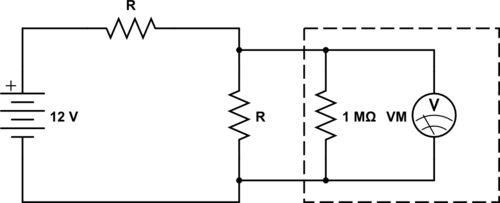
\includegraphics{1_42.png}\\
Assuming the voltmeter is an oscilloscope with a 1-M$\Omega$ input resistance, calculate the voltmeter reading for (a) $R=1k\Omega$ and (b) $R=1M\Omega$.\\
(a)$R=1k\Omega$:\\
The voltage drop across the second resistor will be proportional to the equivalent resistance.  Ex, if $R_{eq}\approx R$\ then $V\approx \frac{12V}{2}$.
$R_{eq}$:
\begin{align*}
R_{eq} &= \frac{1}{\frac{1}{1k\Omega}+\frac{1}{1M\Omega}}\\
R_{eq} &= 999.001\Omega \approx 1k\Omega=R\\
V=I_1R_1+I_2R_2, I_1=I_2, V&=12V\\
1k\Omega I+ .999k\Omega I&=12V\\
I&=\frac{12V}{1.999k\Omega}\approx 6mA\\
\text{Voltmeter reading:}\ V &=I(.999k\Omega)\\
V &= 5.997V \approx 6V
\end{align*}
(b) $R=1M\Omega$:\\
\begin{align*}
R_{eq} &= \frac{1}{\frac{1}{1M\Omega}+\frac{1}{1M\Omega}}\\
R_{eq} &= 0.5M\Omega\\
V=I_1R_1+I_2R_2, I_1=I_2, V&=12V\\
1M\Omega I+ 0.5M\Omega I&=12V\\
I&=\frac{12V}{1.5M\Omega}= 8\mu A\\
\text{Voltmeter reading:}\ V &=I(0.5M\Omega)\\
V &= 4V
\end{align*}

\section*{Circuit Diagrams}
Resistor:\\
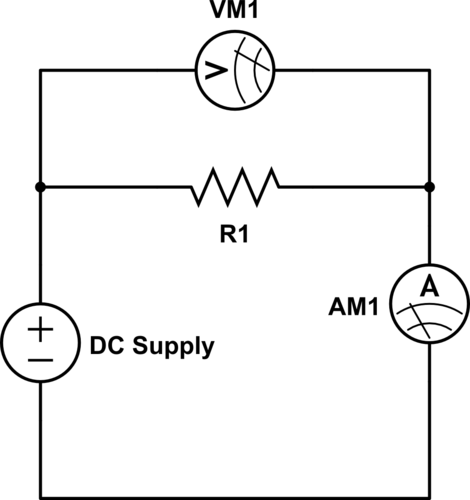
\includegraphics{lab-1-circuit-1c.png}\\
Graphite:\\
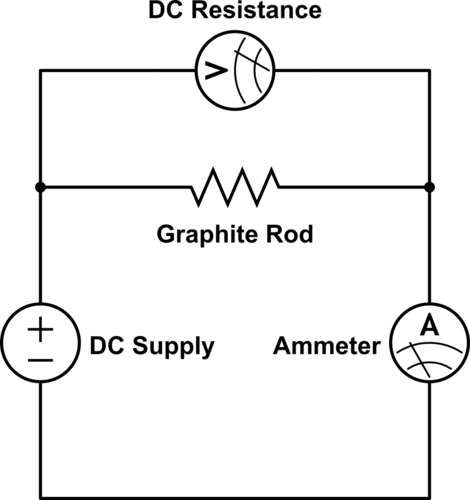
\includegraphics{graphite-rod.png}\pagebreak\\
Diode:\\
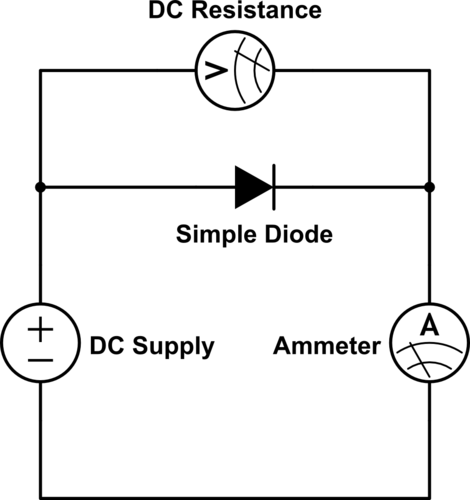
\includegraphics{simple-diode.png}\\
LED:\\
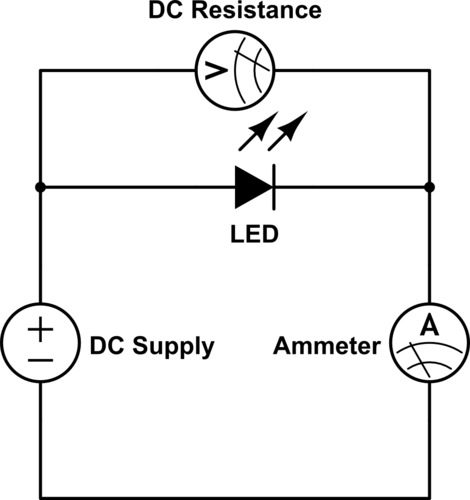
\includegraphics{led.png}\pagebreak\\
Resistor Thermal Check:\\
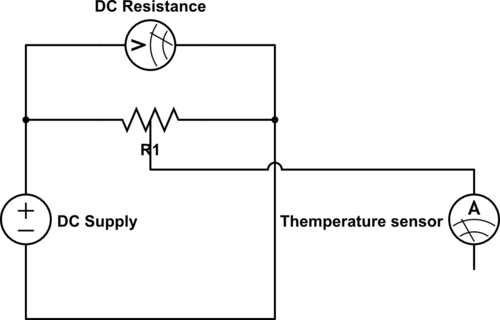
\includegraphics{temp-circuit-1.png}\\
Thermister:\\
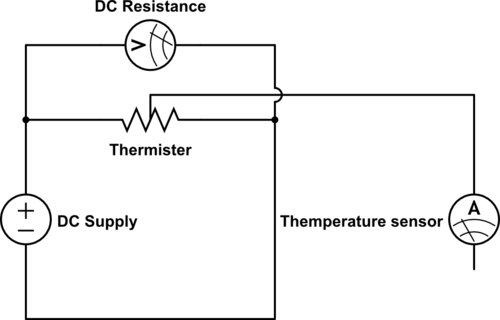
\includegraphics{thermister.png}\pagebreak\\
Potential-divider:\\
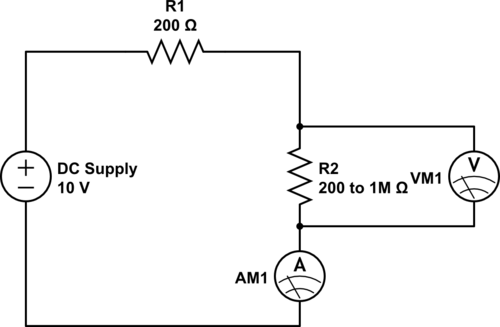
\includegraphics{potential-divider.png}\\
Thevinin-Complex:\\
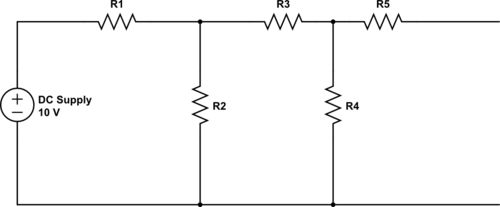
\includegraphics{complex.png}\\
\section*{Data Tables}
1c:\\
\csvautotabular{411labp1.csv}\pagebreak\\
1d:\\
\csvautotabular{411labp1d.csv}\pagebreak\\
1e:\\
\csvautotabular{411labp1e.csv}\\
2a Small Rod:\\
\csvautotabular{411labp2asmall.csv}\\
2a Big Rod:\\
\csvautotabular{411labp2abig.csv}\pagebreak\\
2b:\\
\csvautotabular{411labp2b.csv}\pagebreak\\
2c:\\
\csvautotabular{411labp2c.csv}\\
3a:\\
\csvautotabular{411labp3a.csv}\pagebreak\\
3b:\\
\csvautotabular{411labp3b.csv}
\end{document}
